
Der Einsatz generativer KI erstreckt sich inzwischen über zahlreiche
Unternehmensbereiche hinweg und ist längst nicht mehr auf die reine
Softwareentwicklung beschränkt. Besonders häufig finden entsprechende Tools
Anwendung in der Softwareentwicklung, im Marketing und im Kundensupport, wie
aktuelle Daten zeigen (siehe Abbildung~\ref{fig:ki-einsatzbereiche}). Dies
verdeutlicht, dass generative KI-Tools vielfältig eingesetzt werden und bereits
in unterschiedlichen Domänen signifikante Mehrwerte generieren.

\begin{figure}[H]
    \centering
    \vspace{1em}
    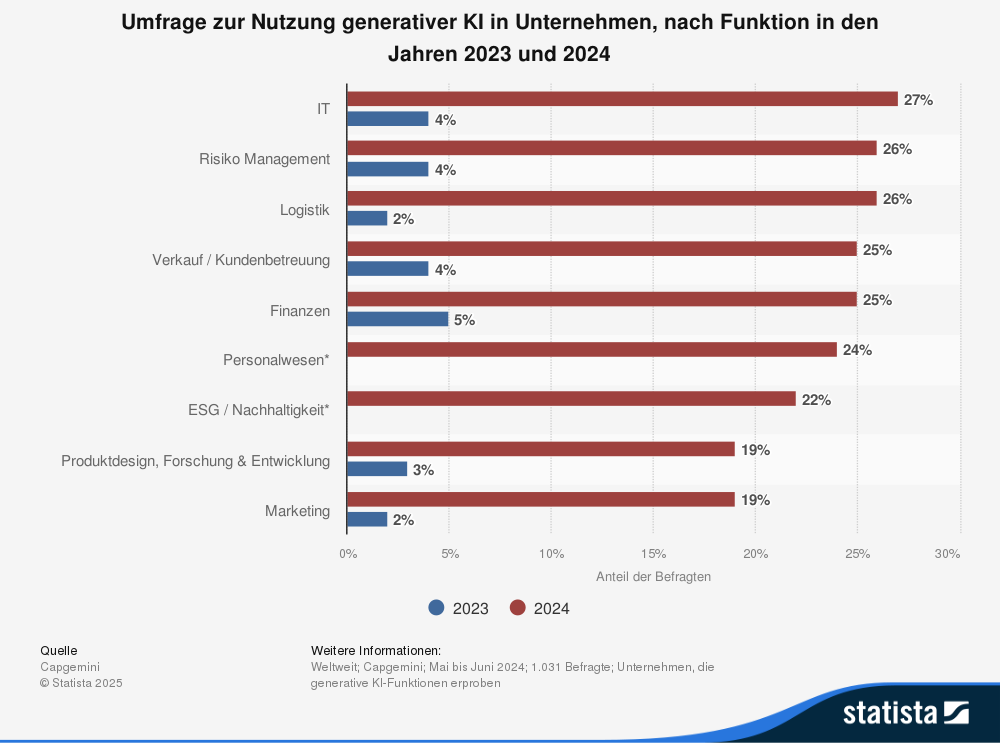
\includegraphics[width=0.7\textwidth]{images/abbildungen/statistic_id1483724_nutzung-generativer-ki-in-unternehmen-nach-bereich-2024.png}
    \caption{Nutzung generativer KI in Unternehmen nach Bereich (2024). Quelle: Capgemini~\cite{statista_ki_einsatzbereiche_2024}.}
    \label{fig:ki-einsatzbereiche}
\end{figure}

Der verstärkte Einsatz generativer KI hat in den letzten Jahren eine Vielzahl
neuer Werkzeuge und Methoden in der Softwareentwicklung hervorgebracht.
Besonders die Integration von Large Language Models (LLMs) in moderne
Entwicklungsumgebungen hat die Arbeitsweise von Entwickler:innen grundlegend
verändert~\cite{esposito_generative_2025,nguyen-duc_generative_2023}. Zu den
zentralen Tools zählen \textbf{GitHub Copilot}, \textbf{Cursor AI},
\textbf{Amazon CodeWhisperer} und \textbf{Devin AI}. Diese werden in der
Literatur umfassend behandelt und spielen laut Esposito et
al.~\cite{esposito_generative_2025} und Nguyen-Duc et
al.~\cite{nguyen-duc_generative_2023} eine Schlüsselrolle in der aktuellen
Entwicklungspraxis. GitHub Copilot unterstützt insbesondere bei der
automatischen Codegenerierung und Vervollständigung und kommt zunehmend bereits
in frühen Phasen wie der Anforderungsanalyse oder der Erstellung von
Architekturentwürfen zum Einsatz.

Moderne Tools wie Cursor AI ermöglichen darüber hinaus dialogorientierte
Workflows, in denen nicht nur einzelne Codezeilen, sondern ganze Features oder
Projekte automatisch erstellt und iterativ optimiert werden können. Methoden
wie Prompt Engineering, Retrieval-Augmented Generation (RAG) sowie
agentenbasierte Ansätze kommen hier zum
Einsatz~\cite{esposito_generative_2025}. Gleichzeitig zeigen aktuelle Studien
auch Grenzen auf, etwa Diskrepanzen zwischen Erwartungen an die
Testautomatisierung und der tatsächlichen
Umsetzbarkeit~\cite{karhu_expectations_2025}, oder Herausforderungen bei
multimodaler KI in der Aufwandsschätzung~\cite{islam_multimodal_2025}.

Die Einführung dieser Werkzeuge und Methoden wird in zahlreichen Publikationen
diskutiert. So beschreibt Kerr~\cite{kerr_github_nodate} praxisnah die
Integration von Copilot, während Weisz et al.~\cite{weisz_design_2024}
Designprinzipien für den produktiven Einsatz formulieren. Weitere aktuelle
Themen sind Prompt Engineering, dialogbasierte Workflows und flexible, agile
Prozesse~\cite{nguyen-duc_generative_2023,gill_agile_2025}. Erfahrungen aus der
Praxis, wie sie von Rogachev~\cite{rogachev_my_nodate} beschrieben werden,
bestätigen zudem, dass die Kombination dieser Ansätze Produktivität und
Codequalität nachhaltig verbessert.

Generative KI-Systeme werden heute nicht mehr nur als reine
Automatisierungstools gesehen, sondern zunehmend als kreative Partner, die neue
Formen der kollaborativen Ideenfindung und Gestaltung
ermöglichen~\cite{khan_beyond_2025}. Besonders im Zusammenspiel verschiedener
Tools zeigen sich erhebliche Produktivitätsgewinne, wie auch die im Praxisteil
(Kapitel~3) dokumentierten Erfahrungen unterstreichen. So konnten insbesondere
durch die Kombination von Tools wie Copilot, Cursor und Bolt Effizienzgewinne
beim schnellen Prototyping, bei Standardaufgaben wie Boilerplate und bei der
automatischen Testgenerierung erzielt werden. Die Fähigkeit,
Kontextinformationen, etwa durch Screenshots oder Fehlermeldungen, direkt in
den Entwicklungsprozess einzubinden, erwies sich zudem als entscheidender
Vorteil beim Debugging und in iterativen Workflows.

Neben den genannten Werkzeugen haben sich auch neue Methoden in der
Entwicklungspraxis etabliert:
\begin{itemize}
    \item \textbf{Prompt Engineering:} Anforderungen werden in natürlicher Sprache formuliert und direkt von der KI interpretiert~\cite{esposito_generative_2025}.
    \item \textbf{Retrieval-Augmented Generation (RAG):} KI-Tools kombinieren projektspezifische Kontextdaten mit aktuellen Benutzeranfragen, um passgenaue Lösungen zu generieren~\cite{esposito_generative_2025}.
    \item \textbf{Human-in-the-Loop und Pair Programming:} Die Zusammenarbeit von Mensch und KI (z.\,B. über Feedback-Loops) gewinnt an Bedeutung, um Qualität und Anpassungsfähigkeit der Entwicklung zu sichern~\cite{nguyen-duc_generative_2023,siebert_generative_2024}. J et al.~\cite{j_integration_2023} zeigen, dass insbesondere bei der Automatisierung von Routineaufgaben KI-Tools signifikante Vorteile bieten und zunehmend als Standardwerkzeuge in agilen Teams akzeptiert werden.
\end{itemize}

Der Blog des Fraunhofer IESE~\cite{siebert_generative_2024} betont, dass
moderne KI-Tools längst über reine Autovervollständigung hinausgehen und
zunehmend Aufgaben im gesamten Entwicklungsprozess übernehmen, von der
Testgenerierung bis zum Refactoring.